\documentclass[sigconf]{acmart}
\usepackage{xeCJK}
\setCJKmainfont{SimSun}
\setCJKsansfont{SimHei}
\usepackage{graphicx}
\usepackage{booktabs}
\usepackage{amsmath}
\usepackage{url}

\setcopyright{none}
\acmYear{2026}
\settopmatter{printacmref=false, printccs=true, printfolios=true}

\begin{CCSXML}
<ccs2012>
 <concept>
  <concept_id>10002951.10003227.10003351</concept_id>
  <concept_desc>Information systems~Data mining</concept_desc>
  <concept_significance>500</concept_significance>
 </concept>
 <concept>
  <concept_id>10010405.10010455.10010458</concept_id>
  <concept_desc>Applied computing~Economics</concept_desc>
  <concept_significance>500</concept_significance>
 </concept>
 <concept>
  <concept_id>10010147.10010257.10010258.10010262</concept_id>
  <concept_desc>Computing methodologies~Learning paradigms</concept_desc>
  <concept_significance>300</concept_significance>
 </concept>
</ccs2012>
\end{CCSXML}
\ccsdesc[500]{Information systems~Data mining}
\ccsdesc[500]{Applied computing~Economics}
\ccsdesc[300]{Computing methodologies~Machine learning}

\title{从 IC 检验到负向筛选：全市场 A 股多因子选股模型的可复现实证研究}
\subtitle{From Information Coefficient to Negative Screening: A Reproducible Empirical Study on a Full-Market A-Share Panel}
\author{数据挖掘技术与应用课程项目组}
\affiliation{%
  \institution{中国石油大学（北京）克拉玛依校区}
  \country{中国}
}
\renewcommand{\shortauthors}{课程项目组}

\begin{document}

\begin{abstract}
本文构建一个覆盖 2016--2026 年、5{,}342 只 A 股、9{,}746{,}194 行、42 因子的日频面板，
研究短周期收益排序的可预测性及其可落地形态。模型采用 LightGBM、3 种子 Transformer 与 Ridge 元模型，
在 5 折 Purged + Embargo 交叉验证下取得 IC $0.1041 \pm 0.0094$（五折全正，ICIR 0.820）。
然而十分位结构显示预测力高度集中于最差一档：D1 单档约 $-10\%/$年，D2--D10 几乎平坦，
高流动性半区中 D10 甚至为负——该模型是「避雷器」而非「选股器」。
在 A 股无法融券做空个股的约束下，唯一可执行形态是剔除打分垫底 10\% 的负向筛选，
三段互不重叠区间年化超额 $+5.85\%$、$+4.67\%$、$+2.87\%$（封存段，一次性）。
我们进一步报告 8 条被证伪的建模路径、三类文本/事件切法的无效性，
以及一个通过严格 CV 增量门的外来因子（缠论中枢位置，$\Delta\mathrm{IC}=+0.0153$，配对 $t=9.92$，0/5 折下降，
三个泄漏探针全部通过）。全部结论、负结果、35 项单元测试与运行日志均可追溯，
并给出从原始数据到最终图表的一键复现流程。
\end{abstract}

\keywords{multi-factor stock selection, purged cross-validation, negative screening, A-share market,
leakage control, reproducibility, factor incrementality}

\maketitle

\section{引言}

短周期收益的可预测性是资产定价与数据挖掘共同关心的核心问题。已有研究在美股与 A 股上分别报告了
机器学习模型对截面收益排序的预测能力~\cite{gu2020,ke2017}，但「IC 显著」与「可交易」之间仍隔着数道约束：
交易成本、做空限制、换手约束，以及最容易被忽视的时间序列泄漏。本文的目标不是再提高一点 IC，
而是回答一个端到端的问题：\emph{在真实市场约束下，一个显著的全市场排序模型能落地成什么形态，
其贡献有多大，且这个结论能否被严格复现？}

我们使用公开的行情、财报、业绩预告与 ST 日历构建异构数据面板，以 t 日收盘出信号、t+1 日收盘买入、
持有 5 日的超额收益为标签，训练并严格验证多因子排序模型。研究贡献有三：

\begin{enumerate}
  \item \textbf{规模与口径}：给出一套覆盖 5{,}342 只股票（含退市名单以抑制幸存者偏差）、
  2{,}622 个交易日、42 因子的后复权面板，并把复权断层、停牌、路径依赖指标的时间对齐
  写成可复用的治理规则。
  \item \textbf{严格的验证纪律}：5 折 Purged + Embargo CV（purge/embargo 各 6 日、expanding 窗口、
  固定轮数不逐折选参）加一次性封存段；所有可训练组件逐折重拟合；任何「加因子」必须过 CV 增量门。
  \item \textbf{负结果与可复现性资产}：系统报告 8 条被证伪路径、事件研究三种切法的无效性、
  以及三类外部因子复现的结论；交付 35 项单元测试、逐脚本运行日志与 4.6 秒可跑通的 Notebook。
\end{enumerate}

\section{相关工作}

\textbf{多因子与机器学习资产定价。} Fama--French 三因子~\cite{fama1993} 与 Amihud 流动性
度量~\cite{amihud2002} 奠定了截面因子框架；Gu 等~\cite{gu2020} 系统比较了机器学习方法在美股
收益预测上的表现。LightGBM~\cite{ke2017} 与 Transformer~\cite{vaswani2017} 分别代表树模型与序列模型
两条主线。本文在此基础上把重点放在 A 股约束下的\emph{落地形态}而非模型容量。

\textbf{金融时序的验证与泄漏。} Purged K-Fold 与 embargo~\cite{lopez2018} 用于处理标签窗口重叠；
本文把该协议扩展到「所有可训练组件逐折重拟合」，并额外处理路径依赖型结构因子的状态映射泄漏。
B6 类的「重复验证」问题（同一批样本被同时标为 dev-val 与 dev-OOS）也在本文中显式排除。

\textbf{可解释性与规则挖掘。} Apriori~\cite{agrawal1994} 与 FP-Growth~\cite{han2000} 用于发现极端状态组合；
SHAP~\cite{lundberg2017} 用于全局与局部归因。持续学习与状态自适应方面，
ReCAP~\cite{pan2026} 提出按市场状态切分并持续更新策略库，本文以独立环境复现其 DOW30 流程作对照。

\section{数据集与数据治理}

\subsection{异构数据源}

\begin{table}[t]
\caption{数据源、形态与规模}
\label{tab:data}
\small
\begin{tabular}{p{2.2cm}p{2.3cm}p{2.0cm}p{1.5cm}}
\toprule
类别 & 形态 & 规模 & 用途 \\
\midrule
后复权日线 & 结构化表格 & 970 万行 & 42 因子 \\
财报与指标 & 结构化表格 & 54 期 $\times$ 4 表 & 基本面 \\
业绩预告 & 半结构化文本 & 91{,}126 条 & 分类、事件 \\
ST / 行业 / 股东 & 结构化表格 & 15 万行以上 & 事件、画像 \\
\bottomrule
\end{tabular}
\end{table}

融合后有效记录 9{,}746{,}194 行，主分析表 42 字段，跨 3 张以上表关联；交付 110 字段数据字典
（含缺失率、单位、取值范围、来源与时点）与逐数据集的数据溯源档案。

\begin{figure}[t]
  \centering
  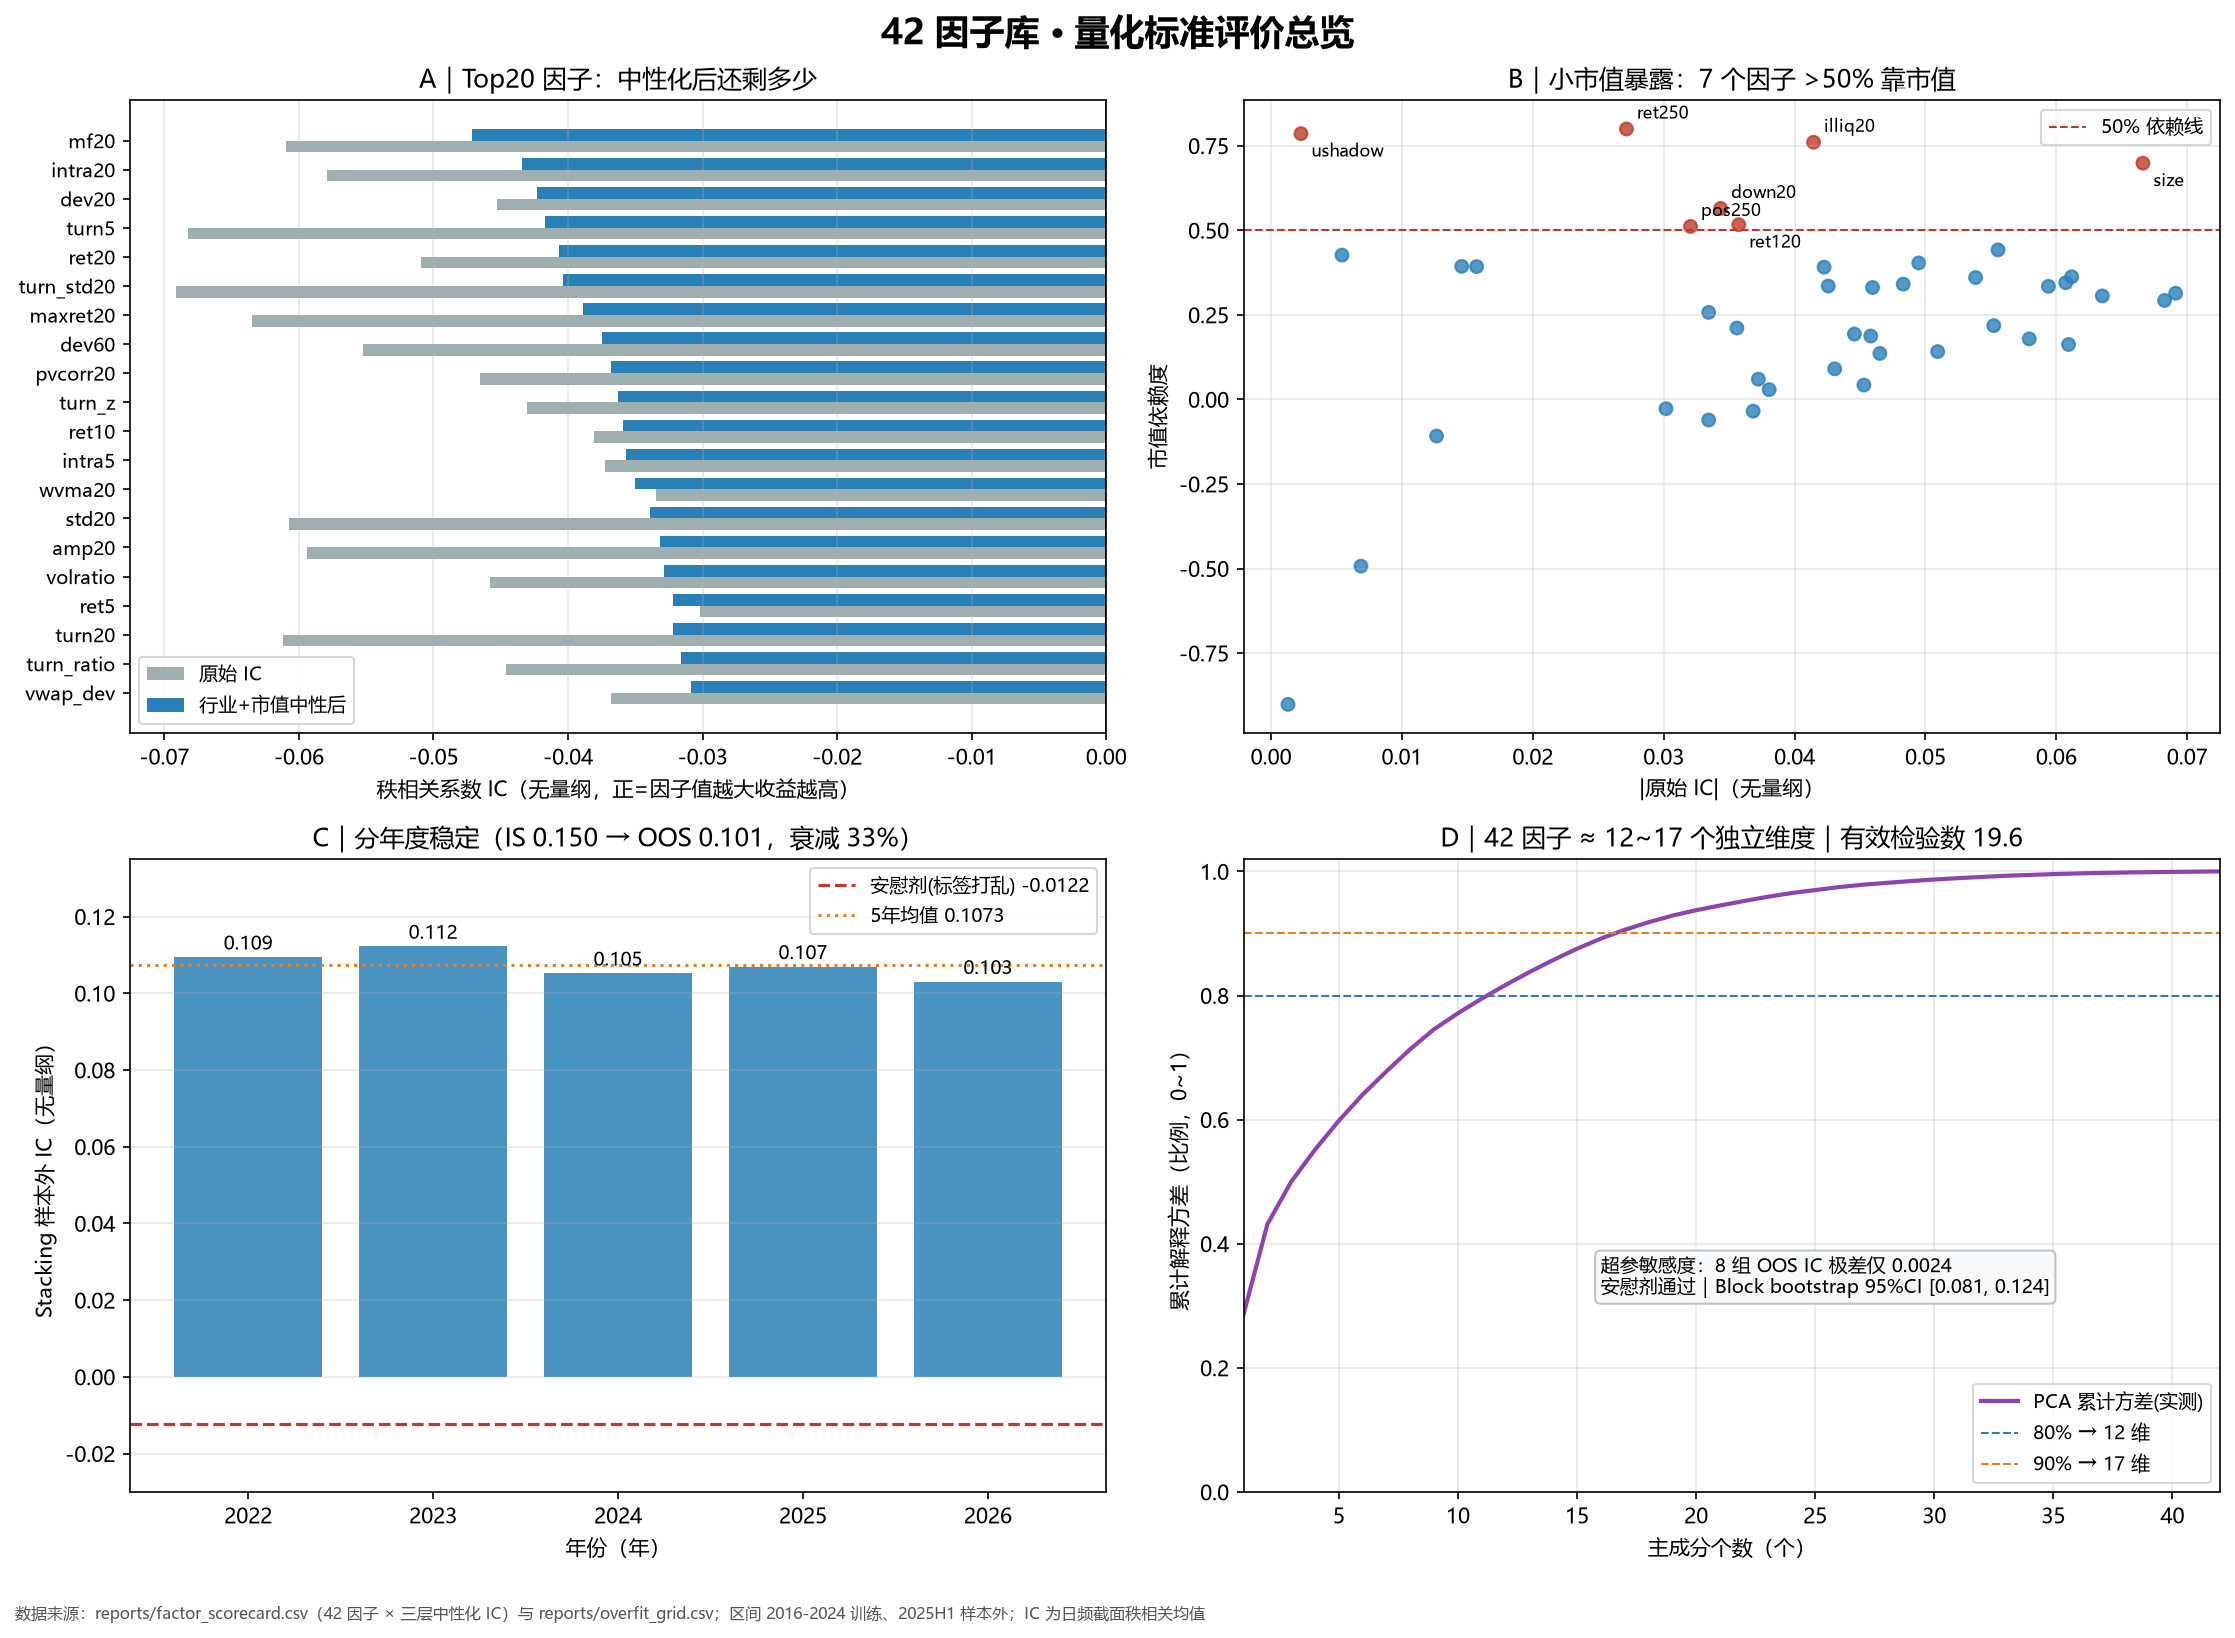
\includegraphics[width=\columnwidth]{../factor_scorecard.png}
  \caption{42 因子打分卡。数据来源：本项目面板，2016--2025。}
  \label{fig:scorecard}
\end{figure}

\subsection{三条决定性口径}

\textbf{后复权（hfq）。} 东财 A 股前复权采用「减法复权」，会把贵州茅台历史价调成 $-143.50$ 元；
负价区间的收益符号反转，足以毁掉全部动量类因子。本项目一律使用后复权。

\textbf{复权断层的制度反查。} 相邻日收益若超出涨跌停制度上限（主板 $\pm10\%$、
创业板 2020-08 后 $\pm20\%$、科创板 $\pm20\%$、北交所 $\pm30\%$）加 2 个百分点，
且不属于新股前 5 日或长停复牌，则判为数据断层。处理分三层：断层日收益置空；
跨断层的 5 日前向标签作废；回看型因子（$ret5/10/20/60/120/250$、$dev20/60$、$pos250$、
$momq60$、$wvma20$）在窗口跨断层时置空。绝对收益统一取自已清洗的收益矩阵，不各自从收盘价重算。

\textbf{防泄漏。} 标签定义为 $Y_2 = close_{t+6}/close_{t+1} - 1$ 后截面去均值；
训练目标用 rank 变换 $(rank - 0.5)/n$。验证采用 6 块 expanding 切分、purge 6 日、embargo 6 日、
5 折；LGBM、Ridge 线性基线、因子 ICIR 权重与 Stacking 元模型全部逐折重拟合；
重采样、标准化、特征选择仅在训练折内进行；封存段 2025-07$\sim$2026-10 只在开发结束后打开一次。

\section{方法}

\subsection{因子与模型}
42 个因子中最强的是资金加权收益 \texttt{mf20}（OOS IC $-0.073$）、成交额扩张
\texttt{amt\_ratio}（$-0.068$）与流动性恶化 \texttt{illiq\_ratio}（$+0.053$）。
增量实验表明：仅 12 个量价因子即达到旧 30 因子集约 92\% 的效力，
合并后 IC 仅提升约 0.003，却使因子合成基线 IC 从 0.0411 升至 0.0550（$+34\%$）。

模型采用 LGBM（best\_iter $=85$）、3 seed Transformer（40 日 $\times$ 42 因子序列）与
Ridge 元模型 Stacking。对照实验显示 rank 回归（IC 0.112）优于 pairwise（0.108）与 BCE（0.084）。
需注意 Stacking 元层在 5 折上为负贡献（$-0.0045$），因此报告只把 dev 段 0.1316 作为内部结果，
不作为独立样本外证据。

\subsection{落地形态与评估指标层级}

评估遵循四级递进判定：\emph{IC $\to$ D1 命中率 $\to$ 全市场 D1 桶 $\to$ 组合年化超额}。
单看代理指标会互相矛盾：某次尾部加权实验在 IC 口径上判为无效（$-0.0003$），
换成 D1 命中率却改善 3.3pp，而全市场对照显示避损反而变差，最终组合年化 $-0.38$pp 且不显著。
因此本文以组合层面的年化超额为终局指标。

落地公式明确为：持有宽基/等权组合，按模型打分剔除垫底 $10\%$，5 日调仓，单边 15bp。
组合超额按 $\frac{n}{N-n}$ 的剔除比例对 D1 与全市场均值之差折算，
避免早期实现中把 $-\mathrm{mean}(D1)$ 直接当年化而虚增到 $+53\%$ 的错误。

\section{实验}

\subsection{主结果}

\begin{table}[t]
\caption{5 折 Purged CV 与 dev 段结果}
\label{tab:cv}
\small
\begin{tabular}{lcc}
\toprule
指标 & 数值 & 备注 \\
\midrule
面板 & 9{,}746{,}194 行 & 2{,}622 日 $\times$ 5{,}342 只 \\
LGBM dev IC & 0.1285 & best\_iter 85 \\
Stacking dev IC & 0.1316 & Ridge 元模型 \\
\textbf{5 折 CV IC} & \textbf{0.1041 $\pm$ 0.0094} & 五折全正 \\
ICIR & 0.820 & 日频 IC 均值/标准差 \\
\bottomrule
\end{tabular}
\end{table}

\begin{figure}[t]
  \centering
  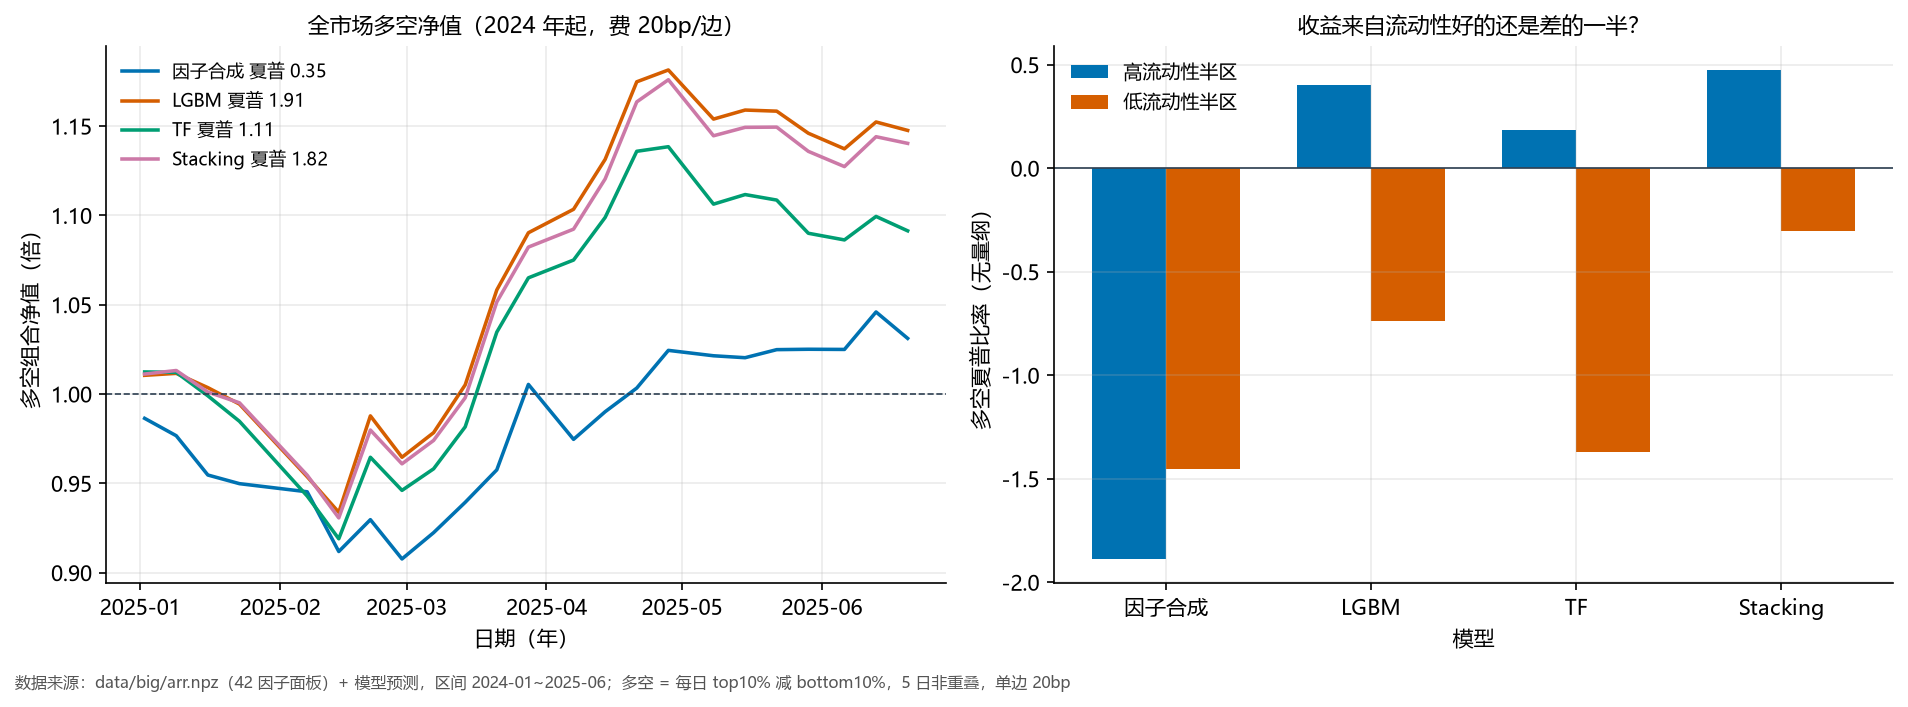
\includegraphics[width=\columnwidth]{../big_eval.png}
  \caption{模型评估：逐折 IC 与多空组合。数据来源：本项目 5 折 CV，2016--2025。}
  \label{fig:eval}
\end{figure}

十分位结构解释了模型本质：D1 单档约 $-10\%/$年，D2--D10 几乎平坦，高流动性半区中 D10 为 $-1\%$。
多空 13pp 价差中约 10pp 来自「避开 D1」。纯多头 top10\% 超额 $-2.9\%\sim-5.4\%$，
而剔除垫底 10\% 的超额为 $+3.3\%\sim+3.7\%$，波动仅 1.7\%。

\subsection{禁买清单：三段互不重叠验证}

\begin{table}[t]
\caption{剔除垫底 10\% 的年化超额（5 日调仓，单边 15bp）}
\label{tab:screen}
\small
\begin{tabular}{lc}
\toprule
区间 & 年化超额 \\
\midrule
2024（meta 段） & $+5.85\%$ \\
2025H1（dev 段） & $+4.67\%$ \\
2025-07 $\sim$ 2026-10（封存段） & $+2.87\%$ \\
\bottomrule
\end{tabular}
\end{table}

三段超额单调衰减，信号在减弱但始终为正。一处口径修正值得记录：原实现用 DataFrame 行索引
计算名单更替，跨日索引不重叠导致每期恒为「100\% 更替」、成本多扣约 1.7bp/期；
改用股票代码后真实更替 44\%，各段数字上修约 0.8pp，旧结果留档可查。

\subsection{数据挖掘方法横向结果}

\textbf{关联规则。} Apriori 与 FP-Growth 产出完全相同的 30 条规则，后者快 4.7 倍。
9 组阈值敏感性分析后，规则按「同前件且后件为子集」去重并剔除平凡规则，归为五族：
偏离均线+高波动（lift 2.49）、振幅扩张+日内强势（2.42）、近期涨停+高于成本（2.40）等。
\texttt{illiq} 在 184 条原始规则中仅出现 9 次，却在 ICIR 线性加权中占 67\% 权重——
线性加权要单调排序、关联规则要极端子集，两者互补。

\textbf{分类。} 在 2{,}398 训练 / 602 评估的公告情感任务上，分层 5 折与超参搜索后：
结构化字段 93.2\% $>$ BERT 89.2\% $>$ LR 88.2\% $>$ Qwen3-0.6B SFT 87.9\%
$>$ 10 行正则 84.6\% $>$ Laya 冻结微调 78.7\%。错误样本解剖显示，
大模型在「正文明确写出预增/预减」的 90\% 样本上输给字符串匹配，
只在「正文不写方向」的 9.5\% 样本上领先（66.7\% vs 47.4\%），瓶颈是任务定义而非容量。
不平衡处理中类别权重最优（macro-F1 0.891，中性召回 0.90），SMOTE 无额外收益。

\textbf{聚类。} 4{,}914 只 $\times$ 42 因子画像，肘部拐点 $k=4$、轮廓系数最优 $k=2$；
高维下轮廓系数随 $k$ 单调下降，故以 bootstrap ARI 裁决：$k=4$ 时 0.963（稳定），
$k=31$ 时仅 0.392——现用行业 31 组在重抽样下约三分之一标签会变。

\begin{figure}[t]
  \centering
  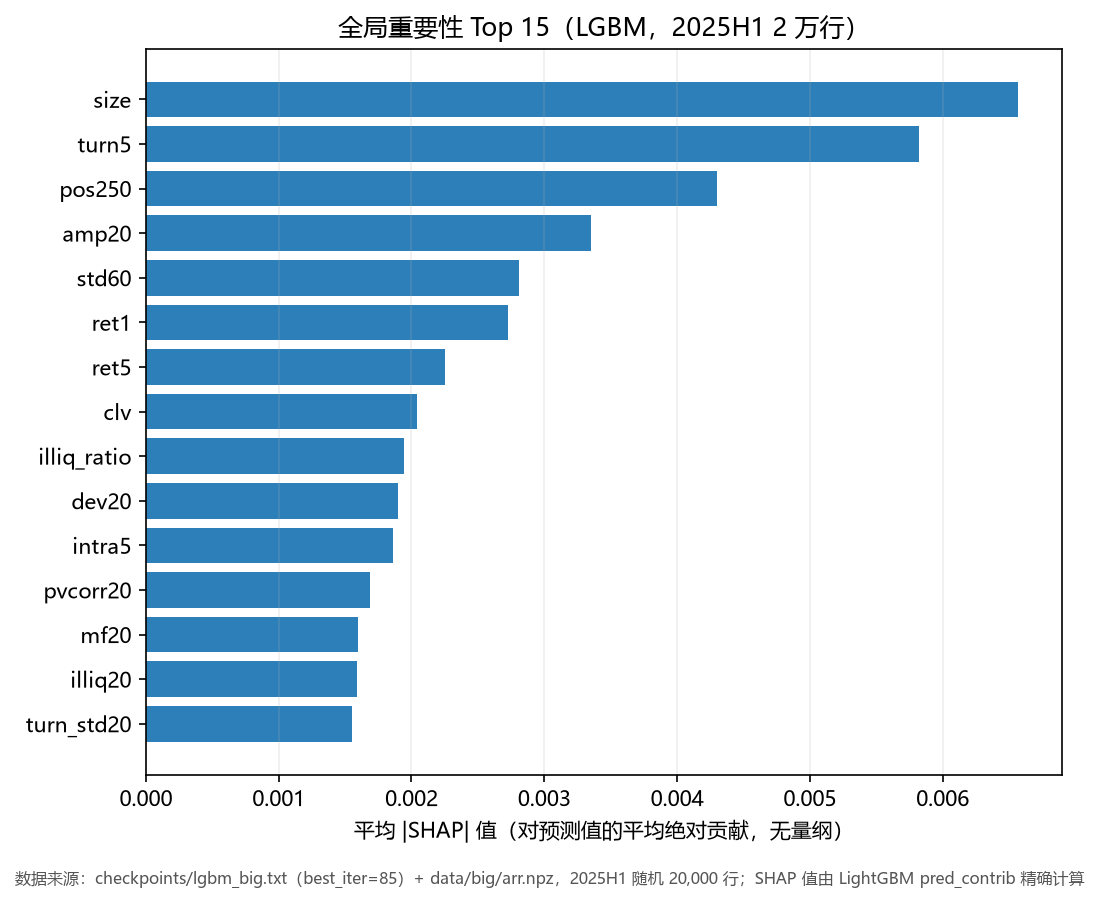
\includegraphics[width=\columnwidth]{../shap_global.png}
  \caption{SHAP 全局重要性。市值 11.6\%、5 日换手 10.3\%、250 日位置 7.6\%。
  数据来源：本项目 LGBM TreeSHAP。}
  \label{fig:shap}
\end{figure}

\textbf{可解释性。} 全局前三为 \texttt{size} 11.6\%、\texttt{turn5} 10.3\%、\texttt{pos250} 7.6\%；
线性口径给 \texttt{illiq\_ratio} 36.9\% 权重，SHAP 中仅排第 9（3.4\%）。
这一差异说明树模型主要把流动性维度用于交互而非主效应。

\textbf{事件研究。} 采用 CAR + 同股票安慰剂分位 + 同侪对照三件套：
财报 SUE 极端 5 日 CAR $-1.49\%$（$t=-2.62$），业绩预告 $-0.58\%$（$t=-0.83$），
ST 摘帽 250 日 CAR $-13\%$ 但安慰剂分位 40\%（非事件效应）。
进一步以「公告 vs 卖方 FY2026 一致预期」偏离度检验 275 个匹配事件，
五分位 Q5$-$Q1 在 5/20/60 日为 $-1.82\%/-1.73\%/-3.39\%$，$p=0.34\sim0.48$ 全不显著。
业绩预告的三种切法（类型、文本、公告 vs 预期）均无交易级超额。

\begin{figure}[t]
  \centering
  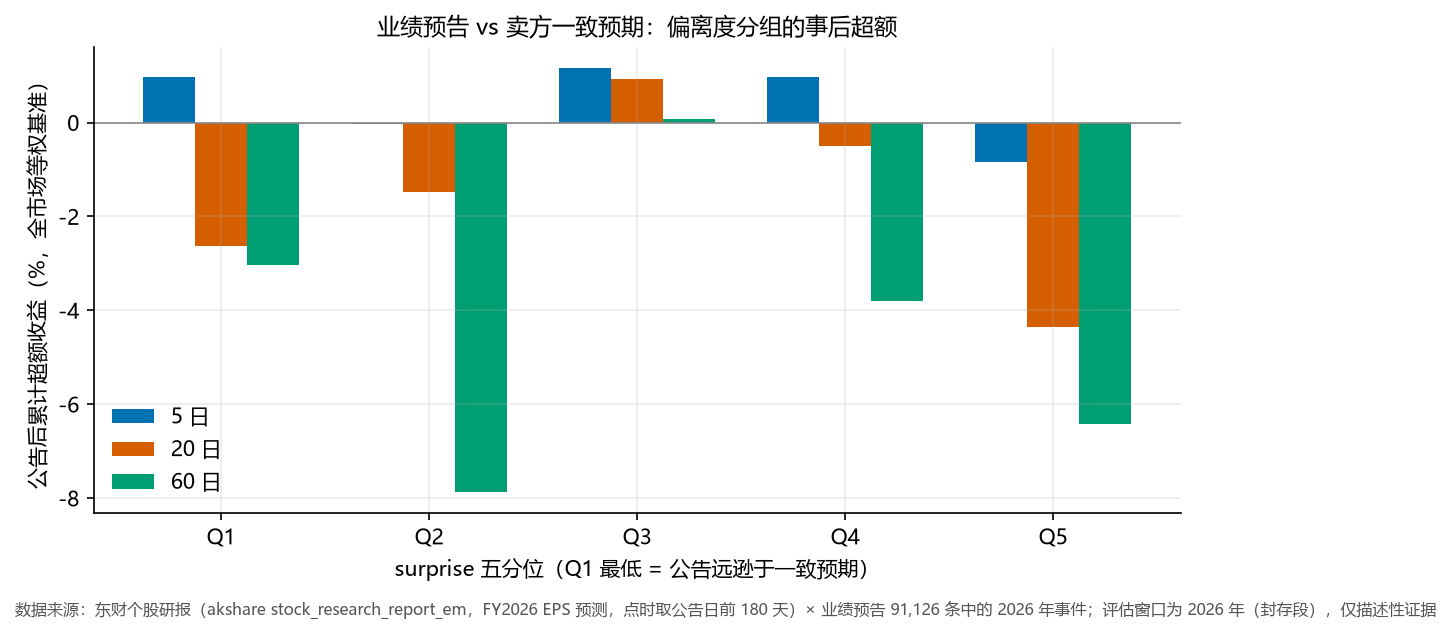
\includegraphics[width=\columnwidth]{../consensus_surprise.png}
  \caption{公告 vs 一致预期偏离度的五分位事后超额。数据来源：东财研报 $\times$ 业绩预告，2026 年。}
  \label{fig:surprise}
\end{figure}

\subsection{因子复现与增量检验}

\begin{table}[t]
\caption{外部因子复现与对照实验}
\label{tab:repro}
\small
\begin{tabular}{p{2.0cm}p{3.4cm}p{2.0cm}}
\toprule
对象 & 做法 & 结论 \\
\midrule
WQ101 价量背离 & 复现 + 相关/增量 & IC 0.051，九成被 \texttt{pvcorr20} 解释，不入库 \\
缠论结构 & 分型/笔/中枢/背驰 + 全市场 5 折 CV & 中枢位置 $\Delta\mathrm{IC}=+0.0153$，$t=9.92$，0/5 折下降 \\
ETF 三因子 & 固定池 vs 事前动态池 & 动态池 $-2.4\%$ vs 固定池 $+10.2\%$，原文系事后挑池 \\
国家队跟随 & 23 期、4 基准 & $-4.6$pp（$p=0.220$），增持信号无效 \\
TAA v3 & 12 变体 + 卫星腿 & 夏普 0.49 vs 0.93，三种用法均不成立 \\
ReCAP (KDD'26) & 独立 venv，DOW30 & 跑通；持续更新使 CR 由 $-99.3\%$ 收窄至 $-55.1\%$ \\
\bottomrule
\end{tabular}
\end{table}

缠论案例值得展开。我们实现合并 K 线 $\to$ 分型 $\to$ 笔 $\to$ 中枢 $\to$ 背驰共 10 个因子。
笔幅度与中枢宽度与既有 \texttt{dev20}/\texttt{std60} 高度相关（0.64），残差归零；
唯一有增量的是「中枢内相对位置」：控制中期动量后残差 IC $+0.0115$、9 年全正、
五分位 Q5$-$Q1 年化 $+15.2\%$。

按项目规矩，加因子必须过 CV 增量门。我们在全市场 5{,}342 只上重算该因子，
以完全相同协议跑三臂：A 基线（42 因子）、B 加原始值、C 加逐日截面回归剔除
\texttt{momq60}/\texttt{ret60} 后的残差。结果 A 逐折 IC 与正式 \texttt{purged\_cv.py}
完全一致（0.1041 $\pm$ 0.0094，验证协议复现无误），B 为 0.1194（$\Delta +0.0153$，
配对 $t=9.92$，0/5 折下降），C 为 0.1086（$\Delta +0.0045$，$t=5.54$）。
由于「好得不像真的」，另做三个泄漏探针：股票维度列置乱与滞后 60 日均使 IC 退回基线
（$\Delta \approx -0.015$），而把因子提前 10 日（覆盖标签窗）使 IC 跳到 0.2843。
三者共同排除对齐泄漏，确认 $+0.0153$ 为真实增量。
条件 IC 拆解进一步显示其价值来自与动量的交互：高动量组内 IC $-0.032$，
低动量组 $-0.004$，而「低动量 $\times$ 站上箱体上沿」为 $+0.014$——
这正是线性因子表达不了、树能切出的结构。该因子目前\textbf{尚未入库}：
入库需重跑全管线并重估禁买清单，而封存段已消耗。

\begin{figure}[t]
  \centering
  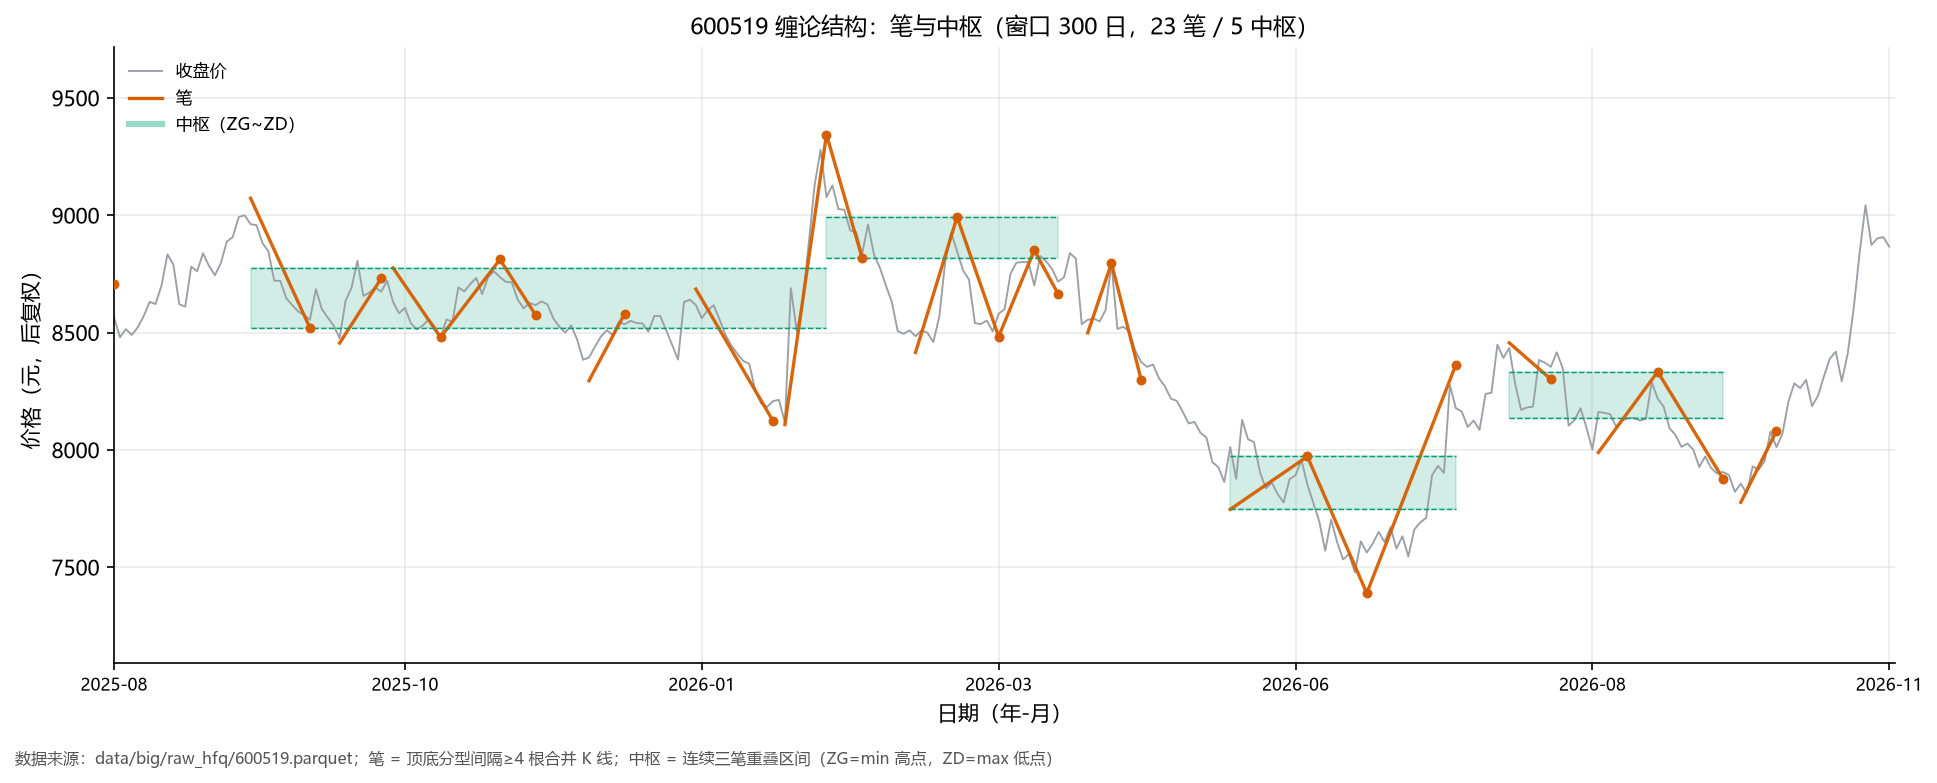
\includegraphics[width=\columnwidth]{../chan_structure.png}
  \caption{缠论结构示意（合并 K 线、分型、笔、中枢）。数据来源：新浪财经日线。}
  \label{fig:chan}
\end{figure}

\begin{figure}[t]
  \centering
  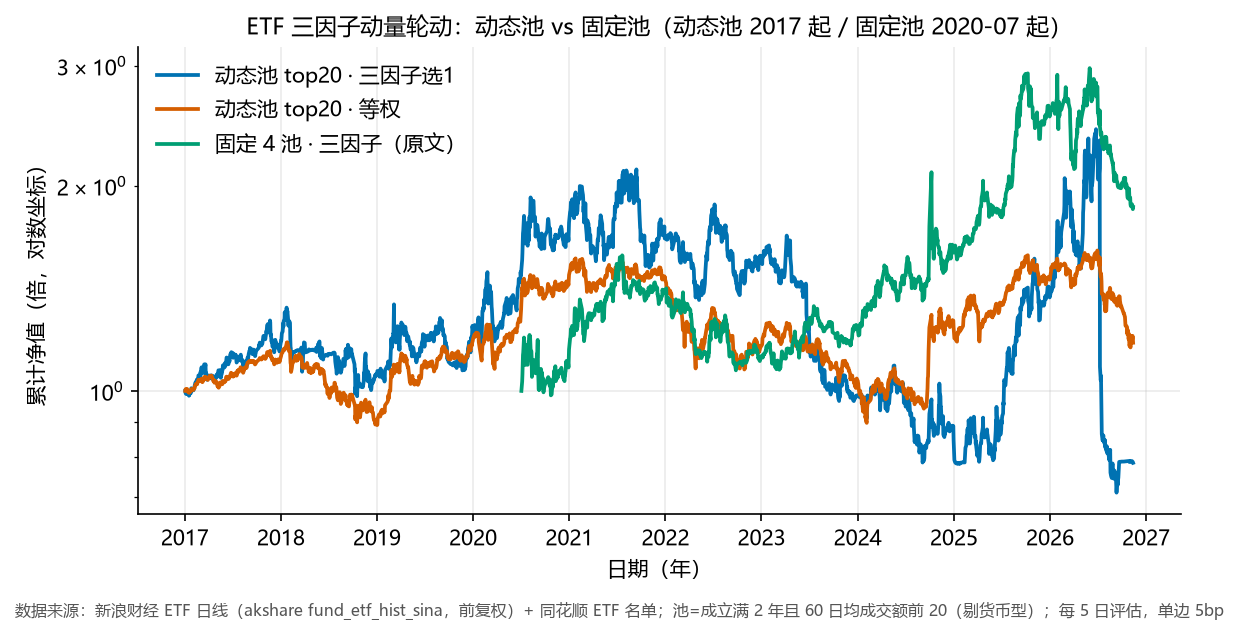
\includegraphics[width=\columnwidth]{../etf_dynamic_pool.png}
  \caption{ETF 三因子动量轮动：动态池与固定池对照。数据来源：新浪 ETF 日线、同花顺名单。}
  \label{fig:etf}
\end{figure}

\subsection{被证伪的路径}

八条路径全部无增量：SVM 日频/截面、多空组合（封存段 $-1.08\%$）、
纯多头 top10\%、行业动量追涨（0 成本 $-5.88\%$/年）、基本面因子加成（5 折中 4 折变差）、
Muon 优化器（与 AdamW 持平）、策略轮动（12 变体全输固定配置）、
行业中性化（申万一级/聚类 31/聚类 4 三种分组均使 CV 下降 0.4$\sim$0.6pp）。
此外记录三处工程教训：合并 K 线组内提前使用状态使残差 IC 从真实 $+0.0115$ 虚增到 $+0.0220$；
SFT 批量生成因右 padding 让 decoder 从填充符续写，准确率仅 11.6\%，逐条生成后 87.9\%；
用当年画像给当年分组造成前视偏差（$+0.1326$ 假象，改上年画像后 $+0.1014$）。

\section{讨论}

为什么模型只能做减法？十分位结构给出的解释是：A 股短周期的可预测性主要来自崩盘风险而非上涨空间。
D1 集中了几乎全部负向信息，而 D10 在高流动性半区甚至掉到 $-1\%$。
这与「个人投资者占比高、壳价值与题材炒作使极端下跌更可预测」的市场结构一致。

为什么必须有多级指标？我们在尾部加权实验中观察到代理指标互相矛盾：
IC 判无效、D1 命中率改善 3.3pp、全市场对照显示避损变差、组合年化 $-0.38$pp 不显著。
只有走到组合层终局指标才能定案。类似地，
「加因子」不能凭单因子 IC 为正就入库，必须做 CV 增量检验——
WQ101 价量背离（IC 0.051）就是反例，而缠论中枢位置（原始 IC $-0.024$）
反倒通过增量门，说明树模型吃的是交互而非线性方向。

\section{效度威胁与局限}

\begin{enumerate}
  \item \textbf{封存段已消耗}：2025-07$\sim$2026-10 的一次性验证已用掉，
  此后任何新模型（包括 43 因子版）无法再做独立验证，只能以 CV 为唯一外部锚。
  \item \textbf{超额衰减}：$+5.85\% \to +4.67\% \to +2.87\%$ 单调下降，信号拥挤度上升。
  \item \textbf{成本假设}：20bp/边能活、50bp/边即 $-31.4\%$/年；实盘应按 30bp 准备，
  且未完整建模涨跌停不可交易与冲击成本。
  \item \textbf{行业口径}：面板存申万二级 128 类，评估统一用申万一级 31 类（覆盖 97.1\%）；
  ARI 0.392 表明细粒度分组不稳定。
  \item \textbf{数据缺口}：减持公告受接口限流不可得，以业绩预告替代；
  卖方一致预期仅覆盖机构关注的标的（12\%），且只有 3 个绝对年份的预测，
  无法构建可靠的点时历史预期面板。
  \item \textbf{文本任务的标签}：公告方向由强制披露字段决定，与「次日超额」标签一致率仅 35.7\%，
  换标签后全部模型准确率 34$\sim$36\%，也说明该文本任务本身信息量有限。
\end{enumerate}

\section{可复现性}

全部 125 个脚本、35 项单元测试（每个对应一个真实 bug）、\texttt{requirements.txt}、
固定随机种子（LGBM seed $=42$、TF 3 seed bagging）、逐脚本运行日志
（时间戳、参数、硬件、耗时、状态）与 4.6 秒可跑通的 Notebook 均随项目交付。
换机器重跑，IC 差 0.0005。完整重跑命令：面板约 40 分钟、训练约 25 分钟、5 折 CV 约 10 分钟。
所有图表统一中文坐标轴、单位、图题与数据来源脚注，采用色盲友好配色。

\begin{verbatim}
python scripts/big_features.py   # 面板
python scripts/big_train.py      # 训练
python scripts/purged_cv.py      # 5 折 CV
python scripts/chan_cv.py        # 因子增量三臂
python scripts/chan_cv_probe.py  # 三个泄漏探针
python scripts/live_screen.py    # 当期禁买清单
\end{verbatim}

\section{结论}

在一个 970 万行、42 因子的全市场 A 股面板上，我们得到 5 折 CV IC $0.1041 \pm 0.0094$，
但证明其预测力集中在最差一档。受做空与成本约束，唯一可落地形态是剔除垫底 10\% 的禁买清单，
年化贡献 $+3\sim5\%$ 且单调衰减。我们系统报告 8 条被证伪路径与多类无效事件切法，
并给出本项目第一个通过 CV 增量门的外来因子及其三个泄漏探针。
本文的核心结论不是「模型有多强」，而是：\emph{在真实约束下，把验证纪律做对之后，
剩下的可交易价值往往只有一点点，且必须靠负向筛选才能兑现。}

\begin{thebibliography}{12}
\bibitem{fama1993} E. F. Fama and K. R. French. 1993. Common risk factors in the returns on stocks and bonds. \emph{Journal of Financial Economics} 33, 1 (1993), 3--56.
\bibitem{amihud2002} Y. Amihud. 2002. Illiquidity and stock returns. \emph{Journal of Financial Markets} 5, 1 (2002), 31--56.
\bibitem{gu2020} S. Gu, B. Kelly, and D. Xiu. 2020. Empirical asset pricing via machine learning. \emph{Review of Financial Studies} 33, 5 (2020), 2223--2273.
\bibitem{ke2017} G. Ke et al. 2017. LightGBM: A highly efficient gradient boosting decision tree. In \emph{NeurIPS}. 3146--3154.
\bibitem{vaswani2017} A. Vaswani et al. 2017. Attention is all you need. In \emph{NeurIPS}. 5998--6008.
\bibitem{lopez2018} M. Lopez de Prado. 2018. \emph{Advances in Financial Machine Learning}. Wiley.
\bibitem{agrawal1994} R. Agrawal and R. Srikant. 1994. Fast algorithms for mining association rules. In \emph{VLDB}. 487--499.
\bibitem{han2000} J. Han, J. Pei, and Y. Yin. 2000. Mining frequent patterns without candidate generation. In \emph{SIGMOD}. 1--12.
\bibitem{lundberg2017} S. M. Lundberg and S.-I. Lee. 2017. A unified approach to interpreting model predictions. In \emph{NeurIPS}. 4765--4774.
\bibitem{devlin2019} J. Devlin et al. 2019. BERT: Pre-training of deep bidirectional transformers. In \emph{NAACL-HLT}. 4171--4186.
\bibitem{kakushadze2016} Z. Kakushadze. 2016. 101 formulaic alphas. \emph{Wilmott Magazine} 84 (2016), 72--81.
\bibitem{pan2026} C. Pan et al. 2026. Regime-Adaptive Continual Learning for Portfolio Management. In \emph{Proc. KDD 2026}. arXiv:2606.00143.
\end{thebibliography}

\end{document}
